\section{Extraction}

Simulink models represent dynamic systems in a number of different ways. Systems can be described through a graphical representation of differential equations (see example in section~\ref{sec:simulink}). Systems can also be described by transfer functions or state machines. Simulink offers many different representational forms. Almost all of these representational forms have in common that they represent \textit{rules} of some sort. When asked to simulate these systems Simulink solves these \textit{rules} in real time and produces the system response. MDPs and POMDPs are much simpler constructs that do not require real-time solvers because the system dynamics is represented as simple state transitions probabilities. Given an MDP or a POMDP representation of a dynamic system, the simulation thereof is merely a question of random sampling.

In order to build these transition probability matrices the \textit{extractor} simulates and observes the given Simulink model multiple times and with different inputs to build up the POMDP's transition probability matrix. In parallel the \textit{extractor} also observes the Simulink model's reward and observation outputs and incrementally builds the reward matrix and the conditional observation probability matrix. The following sections go through the extractor's different functions and discusses them from a high-level point of view.

The chapter ends with two concrete examples that aim to facilitate the understanding of this approach by using real, albeit simple, models and actual numerical values to extract Partially Observable Markov Decision Processes.

\subsection{Approach}
\label{subsec:approach}

The approach chosen for the extraction of Partially Observable Markov Decision Processes from Simulink models is a simple one. If a model is simulated a large enough number of times (see section~\ref{sec:probabilisticsimulation}) from the same source state and given the same action, the transition probability for reaching states in the next step given the source state $s_t = s$ and the action $a_t = a$,
\[
Pr(s_{t+1} = s'|s_t = s, a_t = a),
\]
can be extracted simply by counting the number of times certain sink states, $s_{t+1}$, were reached and normalizing the count vector. This is exactly what the extraction algorithm does for every possible source state given every possible action. In parallel, reward and observation outputs are observed to build the reward model and the conditional observation probabilities described in more detail in sections~\ref{subsec:mdp} and \ref{subsec:pomdp}. The example in section~\ref{subsec:extractexample} presents this process in more detail.

Given a simple input/output model, boundaries for the inputs and boundaries for the outputs, the extractor will extract a POMDP by simulating the model and observing its response. This extraction involves producing actions from input value boundaries, identifying states and building a state space, identifying observations and building an observation space and handling simulation errors and states outside the permitted bounds.

\subsection{Simulink and POMDP Interface}
\label{subsec:extractoveriew}

Using the schematic in figure~\ref{simulinkpomdpinterface}, this section aims to provide an overview of the interfaces between the Simulink model, the extraction algorithm and the Partially Observable Markov Decision Process.

\begin{figure}
\begin{center}
\begin{tikzpicture}[->,>=stealth',shorten >=1pt,auto,node distance=4cm,
                    semithick]
  \tikzstyle{block}=[draw,rectangle,text=black]


  \def\bigrectangle{-- ++(12cm,0cm) -- ++(0cm,7cm) -- ++(-12cm,0cm) -- cycle}
  \def\smallrectangle{-- ++(6cm,0cm) -- ++(0cm,5cm) -- ++(-6cm,0cm) -- cycle}
  \draw[dashed,red] (0,0) \bigrectangle;
  \draw[dotted,blue] (3,1) \smallrectangle;

  \node[red] at (4.0,6.5) {Partially Observable Markov Decision Process};
  \node[blue] at (4.6,5.5) {Simulink Model};
  
  % MDP Inputs
  \node at (-1.1,3.45) {action};
  \draw[->,dashed] (-2.0,3.2) -- (-0.2,3.2);
  \node at (-1.5,5.25) {source-state};
  \draw[->,dashed] (-2.0,5.0) -- (-0.2,5.0);
  \node at (-1.5,1.65) {random input};
  \draw[->,dashed] (-2.0,1.4) -- (2.9,1.4);

  % MDP Outputs
  \node at (13.5,1.25) {reward};
  \draw[->,dashed] (12.2,1.0) -- (14,1.0);
  \node at (13.5,2.95) {observation};
  \draw[->,dashed] (12.2,2.7) -- (14,2.7);
  \node at (13.5,5.15) {sink-state};
  \draw[->,dashed] (12.2,4.9) -- (14,4.9);

  % Simulink Inputs
  \node at (1.65,5.25) {system state};
  \draw[->,dotted] (0.1,5.0) -- (2.9,5.0);

  \node at (2.0,4.25) {input 1};
  \draw[->,dotted] (1,4.0) -- (2.9,4.0);
  \node at (2.0,3.45) {input 2};
  \draw[->,dotted] (1,3.2) -- (2.9,3.2);
  \node at (2.0,2.65) {input 3};
  \draw[->,dotted] (1,2.4) -- (2.9,2.4);
  \draw[-,dotted] (1,2.389) -- (1,4.045);
  \draw[->,dotted] (0.1,3.2) -- (1,3.2);


  % Simulink Outputs
  \node at (9.9,5.95) {output 1};
  \draw[-,dotted] (9.0,5.7) -- (11,5.7);
  \node at (9.9,5.15) {output 2};
  \draw[-,dotted] (9.0,4.9) -- (11,4.9);
  \node at (9.9,4.35) {output 3};
  \draw[-,dotted] (9.0,4.1) -- (11,4.1);
  \draw[-,dotted] (10.96,4.09) -- (10.96,5.745);
  \draw[->,dotted] (10.96,4.9) -- (11.9,4.9);

  \node at (9.9,3.35) {output 4};
  \draw[-,dotted] (9.0,3.1) -- (11,3.1);
  \node at (9.9,2.55) {output 5};
  \draw[-,dotted] (9.0,2.3) -- (11,2.3);
  \draw[-,dotted] (10.96,3.11) -- (10.96,2.255);
  \draw[->,dotted] (10.96,2.7) -- (11.9,2.7);

  \node at (9.9,1.55) {output 6};
  \draw[-,dotted] (9.0,1.3) -- (11,1.3);
  \draw[-,dotted] (10.96,1.310) -- (10.96,0.954);
  \draw[->,dotted] (10.96,1.0) -- (11.9,1.0);

\end{tikzpicture}
\end{center}
\caption{Simulink/POMDP Interfaces}
\label{simulinkpomdpinterface}
\end{figure}

As discussed in section~\ref{subsec:approach}, the extractor works by providing the Simulink model with inputs and observing it's outputs. In order to transform the Simulink model into a POMDP model, Simulink's notion of inputs, outputs and system states must be mapped to the POMDP's base constructs, namely, states, actions, observations and rewards. Figure~\ref{simulinkpomdpinterface} and the rest of this section describe the required transformations between Simulink and POMDP constructs.

On the left side of figure~\ref{simulinkpomdpinterface} one can observe that the extraction algorithm provides three inputs. Firstly it provides a source state and an action and secondly a random number input. The source-state and the action are POMDP constructs, whilst the random input is simply the model's randomness provider (see section~\ref{implextrrand}). Because the Simulink model is based on individual inputs and not on actions, the extraction algorithm must convert the given action into a set of valid Simulink inputs before feeding these to the model. Because the action set is created from the cartesian product of all permitted input values, the action to input transformer simply splits the action into its individual inputs (see section~\ref{subsec:inputsactions} for more details about the action set). Similarily, whilst the POMDP works with state indices, the Simulink model must be provided with an actual Simulink simulation state object. These simulation state objects are saved whenever new states are discovered and the extraction algorithm then merely feeds them back to the Simulink model when the discovered states serve as a source states.

The individual Simulink outputs and their POMDP equivalents can be seen on the other side of figure~\ref{simulinkpomdpinterface}. For the outputs the transformation is inverted, as Simulink outputs must be transformed into POMDP states, observations and rewards. The first $n_s$ outputs are state outputs, meaning that they identify the state the system is in (see section~\ref{subsec:stateoutput}). $n_s$ is an extraction configuration parameter that defines the number of state outputs (see figure~\ref{bw_extract_mdl} for an example of a model prepared for extraction and figure~\ref{exmpl_extract_conf} for an example configuration, showing amongst other things the $n_s$ setting). The next $n_o$ outputs are observation outputs, meaning that they define the observation state. $n_o$ is also a configuration parameter that must be defined before an extraction occurs. The last output is interpreted as the immediate transition reward (see section~\ref{subsec:mdp}) and is taken as-is to build the reward model.

The conversion between POMDP values and Simulink values occurs before and after \textit{every} simulation as the POMDP's conditional transition probability matrix, conditional observation probability matrix and reward model are gradually built.

\subsection{System State and System Output}
\label{subsec:stateoutput}

As described in section~\ref{sec:dynamicsystems} a system's \texti{state} is defined as the smallest possible set of internal and/or external values that represent the system's condition at a certain time. This notion of state in dynamic systems maps exactly onto the idea of states of stochastic processes. Unfortunately an extraction based on applying different inputs to a system and observing it's outputs does not provide \textit{state information} in the above sense, because the relationship between system output and system state is not biconditional. This distinction entails the biggest simplification made by the product of this work, the POMDP extractor.

The extractor does not distinguish between system output and system state as it makes the assumption that \textit{if two system responses are equal the two states of the system are equal}. This simplification was made for two reasons. Firstly, although Simulink offers a way of saving a simulated system's internal state, it does not provide a simple way of comparing two system states. Secondly this simplifications greatly decreases the size of the extracted POMDPs state space. Chapter~\ref{discussion} touches upon the difficulty associated with extremely large state spaces.

A short example may make this rather large simplification clearer. The mathematical pendulum example (see Figure~\ref{1dpendulum}) introduced in section~\ref{sec:dynamicsystems} provides a good basis. As discussed in section~\ref{sec:dynamicsystems} the pendulum system's condition can be described by only two variable, the angular position $\phi(t)$ and the angular velocity $\dot{\phi}(t)$ of the pendulum. Knowing these two values, the system's past can be reconstructed and it's future predicted. If a POMDP extraction of this system were configured with only the angular position $\phi(t)$ as an output, the extractor would interpret the two states,

\begin{align}
 x_{1,t=\tilde{t}} &=\left \begin{pmatrix}
  \phi_1(\tilde{t})=\frac{\pi}{4},\ \dot{\phi_1}(\tilde{t})=0.8\ [\frac{rad}{s}]  \end{pmatrix} \right \nonumber \\
 x_{2,t=\tilde{t}} &=\left \begin{pmatrix}
  \phi_2(\tilde{t})=\frac{\pi}{4},\ \dot{\phi_2}(\tilde{t})=-1.3\ [\frac{rad}{s}] \\
 \end{pmatrix},\right \nonumber
\end{align}

as equal because only the values $\phi_1(\tilde{t})$ and $\phi_2(\tilde{t})$ would be compared. With this simple example the dangers associated with ignoring the ramifications of this simplification become strikingly obvious. The pendulum in state $x_1$ will in the future swing in one direction, whilst the pendulum in state $x_2$ will swing in the opposite direction, clearly a different development, yet deemed equal by the extraction algorithm. In this case the problem could be overcome by defining a second output, the angular velocity $\dot{\phi}(t)$, that would then make the relationship between system state and system output biconditional. With such a configuration the extractor would no longer deem $x_1$ and $x_2$ to be equal system states and thus produce a more realistic POMDP.

A more detailed analysis of the ramifications of this simplification can also be found in chapter~\ref{discussion}.

\subsection{Output Discretization}
\label{subsec:outputdiscretization}

Even though the extraction's source model may be a \textit{continuous} system, the POMDP extractor produces a \textit{discrete} POMDP. In order to extract a discrete POMDP from a continuous model the output values must be discretized, or more accurately quantitized. A simple example would be the sine function system, 
\[
y(t) = sin(x(t)),
\]
where, even though the sine functions codomain is limited, an infinite number of outputs exist. This stems from the fact that the number of values in the range $[-1,1]\in\mathbb{R}$ is infinite in a continuous system. In order to produce a finite state space, the POMDP extractor must thus convert the continous outputs to discrete outputs. This process is sometimes referred to as \textit{binning}, whereby ranges of continuous values are lumped together into a single discretized value.

The quantitization approach chosen for the POMDP extractor is based on \textit{rounding}. For each configured output $i$, the configuration must also contain a rounding parameter $n_i \in \mathbb{Z}$, which is then used to round Simulink output values to the nearest multiple of $10^{n_i}$. This means that given a rounding parameter of $2$, the values $x_1=23.1$, $x_2=3043$, $x_3=100000$ and $x_4=100001$ would be discretized to $\hat{x}_1=0$, $\hat{x}_2=3000$, $\hat{x}_3=100000$ and $\hat{x}_4=100000$, respectively.

The quantitization parameters directly influence the size of the POMDP's state-space and this effect is discussed in more detail in section~\ref{subsec:statediscovery}.

\subsection{Output Boundaries}
\label{subsec:outputboundaries}

The extractor's output is a \textit{finite} POMDP. Simulink models may, on the other hand, have infinite domains. A simple example would be the following system,
\[
y(t) = t,
\]

which obviously has a codomain of the same size as the domain, so potentially infinite. In order to produce a POMDP with a \textit{finite} state space, the extractor requires boundary values for each defined output. Each output value must be given both a minimum and a maximum value that it may not exceed. During the extraction, simulation outputs, and their associated state, are discarded if any one of the output values are outside the defined boundaries.

This approach does however present a problem. During simulations from a single source state given a single action the system response may sometimes lie within and sometimes outside the boundary. This problem is illustrated in table~\ref{outboundssim}, which contains the results of 10 fictitious simulations from the same source state and using the same action. The stochastic dynamic system sometimes responds with values within and sometimes with values outside of the defined output boundaries. Simply ignoring simulations that result in states outside of the defined boundaries would not accurately reflect the system's dynamics.

\begin{table}
\begin{center}
    \begin{tabular}{ | l | l | l | l |}
    \hline
    Simulation Run & Source State & Action & Sink State \\ \hline
    1 & 22 & 6 & 68 \\ \hline
    2 & 22 & 6 & 67 \\ \hline
    3 & 22 & 6 & 122 \\ \hline
    4 & 22 & 6 & out-of-bounds \\ \hline
    5 & 22 & 6 & 68 \\ \hline
    6 & 22 & 6 & 68 \\ \hline
    7 & 22 & 6 & out-of-bounds \\ \hline
    8 & 22 & 6 & out-of-bounds \\ \hline
    9 & 22 & 6 & 67 \\ \hline
    10 & 22 & 6 & 68 \\ \hline

    \end{tabular}
\caption{Simulation with out-of-bounds sink states}
\label{outboundssim}
\end{center}
\end{table}

The solution used by the extraction algorithm is the use of two fictitious states. The first of these is discussed in section~\ref{subsec:simerrors}, but the second one represents exactly the above discussed case of reaching a state with values outside the permitted boundaries. This means that the simulation results of table~\ref{outboundssim} can be interpreted accurately by including the probability of reaching the \textit{out-of-bounds state}. The out-of-bounds state is never used as a source state and has a transition probability of $1$ of not changing for any action. In this case the probability of reaching the out-of-bounds state is:
\[
P(s' = out-of-bounds|s=22,a=6) = 0.3.
\]

The reward gained for reaching the out-of-bounds state must be configured manually in the extrator's parameters.


\subsection{Simulation Errors}
\label{subsec:simerrors}

Similar to the above discussed problem of reaching states outside the permitted boundaries, simulations may also sometimes simply result in errors. Unacceptable input values or combinations thereof, model instability or failed assertions may sometimes lead to simulation errors. Because of the probabilistic nature of the extractor's source models, it is also possible that only a subset of a set of simulations from the same source state and using the same action results in errors. Similarily to the problem of reaching out-of-bounds states, the occurence of errors cannot simply be ignored, but must rather be reflected in the transition probabilities, observation probabilities and reward model of the extracted POMDP.

The solution to this problem is the introduction of a fictitious \textit{error state}. This state does not ever serve as a source state for simulations, but is used as sink state for simulations that fail due to errors. As with the out-of-bounds state discussed in section~\ref{subsec:outputboundaries}, the error state has a transition probability of $1$ not to change for any action. As such, simulation errors can accurately be accounted for in the POMDPs transition probabilities, observation probabilities and reward model.

The reward associated with reaching the fictitious error state is part of the extractor's configuration parameters.

\subsection{Inputs and Actions}
\label{subsec:inputsactions}

MDPs and POMDPs model \textit{controllable} dynamic systems, where a decision taker can influence the system's development over time. Simulink models usually have a single or multiple inputs that are sampled at every time-step and used as input for the given system. In order to extract transition probabilities that depend on the action chosen by the decision maker, simulations must be observed for each of the possible actions. This means that for every state the system may find itself in, simulations must be run with every possible action a decision maker may choose to take. In order to guarantee that the MDP or POMDP will be able to represent the dynamics of the system correctly this means that every possible permutation of permitted input values must be used during the extraction.

A simple example of this can be made with the \textit{ideal gas law} system,
\[
p\cdot V = n \cdot R \cdot T,
\]

where $p\ [Pa]$ is the pressure, $V\ [m^3]$ is the volume, $n\ [mole]$ is the mole quantity, $ R = 8.314\ [J\cdot K^{-1} \cdot mol^{-1}]$ is the universal gas constant and $T\ [K]$ the temperature. Although this system is not dynamic --- it does not change over time --- it is sufficient in this context.

If a conversion of this system to an MDP or a POMDP were necessary with the following configuration,

\begin{itemize}
\item - inputs: pressure $p$, volume $V$, mole quantity $n$,
\item - output: temperature $T$,
\end{itemize}
the action set of an MDP or a POMDP would be defined as the cartesian product of all input sets. If the maximum of each input $x$ were defined as $x_{max}$ and it's minimum as $x_{min}$, the action set would be:

\begin{align}
A &=\left \Pi \times \Lambda \times \Gamma \right \nonumber\\
&=\left \{(p,V,n)\ |\ p\ \in \Pi,\ V  \in \Lambda,\ n \in \Gamma\},\right \nonumber \\
where&\left \right \nonumber \\
\Pi &=\left  [p_{min},(p_{min}+\pi),(p_{min}+2\cdot\pi),\cdots,(p_{min}+(N-1)\cdot\pi),p_{max}] \right \nonumber \\
\Lambda &=\left  [V_{min},(V_{min}+\lambda),(V_{min}+2\cdot\lambda),\cdots,(V_{min}+(N-1)\cdot\lambda),V_{max}] \right \nonumber \\
\Gamma &=\left  [n_{min},(n_{min}+\gamma),(n_{min}+2\cdot\gamma),\cdots,(n_{min}+(N-1)\cdot\gamma),n_{max}] \right \nonumber \\
\pi &=\left \frac{p_{max}-p_{min}}{N_p-1} \right \nonumber \\
\lambda &=\left \frac{V_{max}-V_{min}}{N_V-1} \right \nonumber \\
\gamma &=\left \frac{n_{max}-n_{min}}{N_n-1} \right \nonumber
\end{align}

with $N_i$ being the number of different input values required between the maximum and minimum values of input $x_i$ (see section~\ref{subsubsec:extractionconfig} for an example). The cardinality of $A$ (ie. the number of actions $a \in A$) is

\[
|A| = \prod_{i \in I} N_i.
\]

An example action set with numeric values could be

\begin{align}
 A &=\left \begin{pmatrix}
  (p=0.0,V=0.0,n=0.1) \\
  (p=0.0,V=0.0,n=0.3) \\
  (p=0.0,V=0.0,n=0.5) \\
  \vdots\\
  (p=4.3,V=2.0,n=0.9) \\
  (p=4.3,V=3.0,n=0.1) \\
  (p=4.3,V=3.0,n=0.3) \\
  \vdots\\
  (p=9.9,V=9.0,n=0.5) \\
  (p=9.9,V=9.0,n=0.7) \\
  (p=9.9,V=9.0,n=0.9) \\
 \end{pmatrix}\right \nonumber, \\
 where &=\left \right \nonumber \\
 p_{min} &=\left 0.0,\ p_{max} = 9.9,\ \pi = 0.1    ,\ N_p = 100 \right \nonumber \\
 V_{min} &=\left 0.0,\ V_{max} = 9.0,\ \lambda = 1.0,\ N_V = 10 \right \nonumber \\
 n_{min} &=\left 0.1,\ n_{max} = 0.9,\ \gamma = 0.2 ,\ N_n = 5\right \nonumber
\end{align}

In this case the number of actions comes to 
\[
|A| = \prod_{i \in (p,V,n)} N_i = N_p \cdot N_V \cdot N_n = 100 \cdot 10 \cdot 5 = 5000.
\]

The action set produced in this fashion is then used by the extraction algorithm, described above in sections~\ref{subsec:approach} and~\ref{sec:probabilisticsimulation}.

\subsection{State Discovery}
\label{subsec:statediscovery}

Although the quantitization of an extraction's legal output values completely defines the extracted POMDP's state space, the extractor does not create the n-dimensional state space in advance. The reason for this lies in the difference between the \textit{potential} and the \textit{reachable state space}.

The \textit{potential} state space of a POMDP is defined by the output boundaries and the discretization parameters. The following short example, with two outputs $a$ and $b$ and boundaries, 

\begin{align}
a_{min} &= 0.0 \nonumber\\
a_{max} &= 1.0 \nonumber\\
b_{min} &= 1000 \nonumber\\
b_{max} &= 2000 \nonumber,
\end{align}

illustrates this point. Given these boundaries and discretization parameters the extractor's discretization function may produce the following discrete value buckets for each output,

\begin{align}
a &\in [0.0,0.5,1.0] \nonumber \\
b &\in [1000,2000], \nonumber
\end{align}

meaning that the system could reach the following six states:

\[
x = 
\begin{pmatrix}
x_1 \\
x_2 \\
x_3 \\
x_4 \\
x_5 \\
x_6
\end{pmatrix}
=
\begin{pmatrix}
a = 0.0 & b = 1000 \\
a = 0.0 & b = 2000 \\
a = 0.5 & b = 1000 \\
a = 0.5 & b = 2000 \\
a = 1.0 & b = 1000 \\
a = 1.0 & b = 2000
\end{pmatrix}.
\]

This is the POMDP's \textit{potential state space}, meaning that an extraction may reach all those states but no more. The \textit{reachable} state space is however often much smaller. The limiting factor is the dynamic system itself. Certain systems may never reach some of the states in their potential state space. It may, as a matter of fact, even reach only a tiny subset of it. As such, the extractor is implemented as a \textit{discovering} system that continuously discovers new states and thus builds up its state space gradually.

The only negative consequence of this difference between the \textit{potential} and the \textit{reachable state space} is that only a maximum value prediction can be made of the number of simulations required for an extraction. Experience has, however, shown that the ratio of reachable states to potential states can vary greatly, reducing the value of these maximum time predictions. Such a prediction may be ten years although in reality an extraction may only take a few weeks.

\subsection{Probabilistic Simulations}
\label{sec:probabilisticsimulation}

Markov Processes model probabilistic systems. In order to extract the correct probabilities from the source model, the extractor must run a large enough number of simulations with the same source state and the same action. The number of simulations required to extract the accurate probabilistic nature of the system depends on the system and its inherit randomness. This value cannot be automatically deduced from a system without knowledge of its internal dynamics and must thus be defined as part of the extractor's configuration parameters. The discussion in chapter~\ref{discussion}, discusses the effect of different numbers of simulation runs on the quality of the extracted Markov Process in representing a source model's actual nature.

\subsection{Time Steps and Decision Epochs}
\label{subsec:timestepsdecisionepochs}

Computer simulations occur in artificial time. Although a chemical reaction may take hours, the simulation thereof could take seconds. In order to correctly represent the development of time in relation to the development of a dynamic system, computer simulation use a relative measure of time, so-called \textit{time steps}. The conversion of time steps to real time depends on the model. Certain models may model a minute of real time as a single time steps, whilst other may choose to represent only nano seconds as time steps. This conversion ratio is an inherit property of the model and remains constant for all parts therof. This allows scientists to map simulated changes to changes in reality.

Markov Decision Processes represent time as \textit{decision epochs}. The transitions defined in the conditional transition probabilities matrix introduced in section~\ref{subsec:mdp} occur over a single epoch. Depending on the time granularity of an MDP or a POMDP, a decision epoch may represent a minute, an hour or any other real time value. Section~\ref{subsec:markovprop} discusses in more detail the relationship between the Markov property and the real time length of an artifical decision epoch.

The extraction of MDPs or POMDPs from Simulink models thus requires a conversion between \textit{time steps} and \textit{decision epochs}. The approach to this conversion is simple, yet its ramifications significant (see section~\ref{subsec:markovprop}). The extactor required a simple integer conversion value between time steps and decision epochs. The most granular extraction occurs with a conversion rate of $1$, whereby a single decision epoch represents a single simulation time step. Greater conversion values mean that multiple time steps represent a single decision epoch in the extracted POMDP.

Although the implementation of this conversion is simple the conversion ratio can strongly influence the dynamics of the extracted system.

\subsection{Markov Property and Model Time Lag}
\label{subsec:markovprop}

The Markov Property was introduced in section~\ref{subsec:markovchains}. It states that a Markov Chain's transition probabilities at time $t$ depend only on the state at time $t-1$. Formally it is defined as:

\[
Pr(X_{n+1}=x|X_1=x_1,X_2=x_2,...,X_n=x_n) = Pr(X_{n+1}=x|X_n=x_n).
\]

\begin{figure}
\begin{center}
\begin{tikzpicture}[>=stealth',shorten >=1pt,auto,node distance=4cm,
                    semithick,every text node part/.style={align=center}]
  \tikzstyle{node}=[draw,circle,text=black,minimum size=1.5cm]

  \node [node] at (-1.5,1) {$s_{t-1,1}$};
  \node [node] at (1.5,1) {$s_{t-1,2}$};  

  \node [node] at (0,-2) {$s_{t}$};

  \node [node] at (-3,-5) {$s_{t+1,1}$};
  \node [node] at (0,-5) {$s_{t+1,2}$};  
  \node [node] at (3,-5) {$s_{t+1,3}$};  
  
  \draw[->] (-1.2,0.2) -- (-0.4,-1.3);
  \draw[->] (1.2,0.2) -- (0.4,-1.3);

  \draw[line,dashed] (-5,-0.5) -- (5,-0.5);

  \draw[->,dotted] (-0.8,-2.7) -- (-2.6,-4.2);
  \draw[->,dotted] (0,-2.9) -- (0,-4.2);
  \draw[->,dotted] (0.8,-2.7) -- (2.6,-4.2);
  
\end{tikzpicture}
\end{center}
\caption{Markov Property}
\label{markovproperty}
\end{figure}

Figure~\ref{markovproperty} shows an MDP or POMDP development over three \textit{epochs}. The system may have been in state $s_{t-1,1}$ or state $s_{t-1,2}$ at time $t-1$. It then progresses to state $s_t$ at time $t$ and finally transitions to either state $s_{t+1,1}$, $s_{t+1,2}$ or $s_{t+1,3}$. The Markov property takes action at time $t$, marked by the dashed line, by guaranteeing that the transition probabilities for the state transition between times $t$ and $t+1$ are not affected by whether the system was in state $s_{t-1,1}$ or $s_{t-1,2}$ at time $t-1$; the transition probabilities depend only on the current state $s_t$.

This property has some effect on the extraction of MDPs and POMDPs from Simulink models. In fact, it produces a minimum epoch length for an extracted Markov Process. If the output or state of a Simulink model at time $t$ depends on the model's state at time $t-\tau$, $\tau$ is the minimum length of an extracted Markov Process's epoch. This stems from the Markov Process's Markov Property. If the Markov Process is to correctly represent the dynamics of the system, the epoch must be longer than the maximum time lag inherit in the system.

This limitation must be considered when specifying the ratio between simulation time steps and decision epochs touched upon in section~\ref{subsec:timestepsdecisionepochs}. In order to correctly transfer the system dynamics of the Simulink source model to the extracted Markov Process \textit{the decision epoch must be at least as long as the model's maximum time lag}, otherwise the system's dependence on historical state would not be correctly represented.

A simple example is the following discrete-time system defined as a difference equation:

\begin{align}
y[t] &= \sum_{k=1}^{5} y[t-k] + \sum_{k=2}^{4} x[t-k] \nonumber \\
     &= y[t-1] + y[t-2] + y[t-3] + y[t-4] + y[t-5] + x[t-2] + x[t-3] + x[t-4] \nonumber
\end{align}     

This system depends on past output values as well as past input values, ie. is it not \textit{memoryless}. The maximum time lag is $5$ as the system output at time $t$ depends on the output value at time $t-5$. Coming back to the Markov Property, this means that the minimum conversion ratio between an extracted Markov Process's decision epoch and a simulation time step is $1=\frac{5\ time\ steps}{1\ decision\ epoch}$.

This limitation does not hinder the correct representation of a source system's dynamics as a Markov Process, but it does limit the time granularity of the resulting stochastic process. Not taking model time lags into account when defining the time-step/decision-epoch ratio will however lead to an incorrect transformation and must thus be kept in mind when defining extraction parameters.

\subsection{Example 1: Inputs and Outputs}
\label{subsec:ioexample}

The purpose of this section is to provide an example that will present the simulation, observation and extraction process, especially in terms of simulation inputs and simulation outputs, in a more concrete way. This IO interface has already been introduced in section~\ref{subsec:extractoveriew} and this example builds upon that introduction.

\subsubsection{Model}
\label{ex1model}

The model used as an extraction base is depicted in figure~\ref{ioexamplemodel}. Two things are noticable. Firstly the model is deterministic. No random numbers are used, meaning that the model is referentially transparent, \textit{given the same inputs and source state it will always respond in the same way}. Secondly, the model is source-state-independent. The lack of integrator, time-delay or other state dependent blocks means that the output of the model is entirely independent of the system's current state, it depends only on the actions. Nonetheless, this simple model can serve as an example that depicts the simulation process.

\begin{figure}
\begin{center}
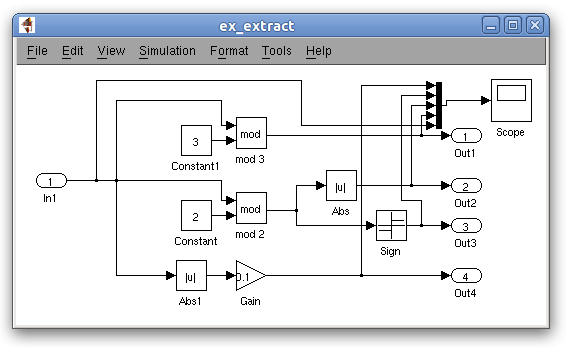
\includegraphics[height=9cm]{media/ex_extract.png}\\
\end{center}
\caption{Simulink Model for Example 1}
\label{ioexamplemodel}
\end{figure}

The model can also be defined formally,

\begin{align}
y_1(t) &= u(t)\ mod\ 3 \nonumber \\
y_2(t) &= |u(t)\ mod\ 2| \nonumber \\
y_3(t) &= sgn(u(t)\ mod\ 2) \nonumber \\
y_4(t) &= \frac{1}{10}|u(t)| \nonumber
\end{align}

where $u(t)$ is the input value at time $t$ and $y_1(t)$, $y_2(t)$, $y_3(t)$, and $y_4(t)$ are the four outputs at time $t$, visible on the left and right side of figure~\ref{ioexamplemodel}, respectively.

\subsubsection{Inputs and Actions}

The actions space is quite small and taken as predefined (see the second example in the next section for a closer look at how the action space is built):

\[
A = \begin{pmatrix}
  a_1 \\ a_2 \\ a_3 \\ a_4 \\ a_5
\end{pmatrix}
 = \begin{pmatrix}
 u = -2 \\ u = -1 \\ u = 0 \\ u = 1 \\ u = 2
 \end{pmatrix}
\]

\subsubsection{Outputs}



The mapping of the POMDP actions to Simulink inputs and Simulink outputs to POMDP constructs, dicussed in section~\ref{subsec:extractoveriew}, is defined as:

\begin{itemize}
\item `In 1': POMDP action value 1
\item `Out 1': POMDP state output 1
\item `Out 2': POMDP observation output 1
\item `Out 3': POMDP observation output 2
\item `Out 4': POMDP reward output 1
\end{itemize}

This means, that Markov Process states represent the value of the first Simulink output, that the observation is a combination of the second and third output and, finally, that the reward is obtained from the last Simulink output.

\subsubsection{State Space}

In order to keep this example simple, no output value boundaries have been defined. As will become obvious, these are not necessary for this example.

\subsubsection{Simulations}

After the action set has been defined, the inputs mapped to actions and the outputs mapped to either state, observation or reward outputs, the extraction can begin. Because of the deterministic nature of this model, each simulation with the same input will always lead to the same outputs. This is why, this example runs but a single simulation for each source-state/action tuple. In reality hundreds of such simulations would be completed in order to observe the model's stochastic behaviour (see section~\ref{sec:probabilisticsimulation}). The simulations presented here are also source state independent. As discussed in section~\ref{ex1model} above, the model's output does not depend on the source state, meaning that the current state of the system does not influence the output.

Table~\ref{ex1simres} shows the inputs used for, and the results produced by all simulations that were run during the extraction.

\begin{table}
\begin{center}
    \begin{tabular}{ | l | l | l | l | l | l | l |}
    \hline
Source State & Action & Inputs & Outputs ($y_1$,$y_2$,$y_3$,$y_4$) & State      & Observation      & Reward \\ \hline
    n/a      & $a_1$  & ($u=-2$)     & $(-2,0,0,0.2)$                    & $(y_1=-2)$ & $(y_2=0,y_3=0)$  & $(y_4=0.2)$ \\ \hline
    n/a      & $a_2$  & ($u=-1$)     & $(-1,1,-1,0.1)$                   & $(y_1=-1)$ & $(y_2=1,y_3=-1)$ & $(y_4=0.1)$ \\ \hline
    n/a      & $a_3$  & ($u=0$)      & $(0,0,0,0)$                       & $(y_1=0)$  & $(y_2=0,y_3=0)$  & $(y_4=0.0)$ \\ \hline
    n/a      & $a_4$  & ($u=1$)      & $(1,1,1,0.1)$                     & $(y_1=1)$  & $(y_2=1,y_3=1)$  & $(y_4=0.1)$ \\ \hline
    n/a      & $a_5$  & ($u=2$)      & $(2,0,0,0.2)$                     & $(y_1=2)$  & $(y_2=0,y_3=0)$  & $(y_4=0.2)$ \\ \hline
\end{tabular}
\caption{Example 1: simulation results}
\label{ex1simres}
\end{center}
\end{table}


\subsubsection{Interpretation}

Given the above simulation results, the state space can now be defined as,
\[
S = \begin{pmatrix}
s_1 = 0 \\
s_2 = 1 \\
s_3 = 2 \\
s_4 = -1 \\
s_5 = -2
\end{pmatrix},
\]

and the discovered observation space as,

\[
O = \begin{pmatrix}
o_1 \\
o_2 \\
o_3
\end{pmatrix}
= \begin{pmatrix}
o_{1,1} = 0, o_{1,2} = 0 \\
o_{2,1} = 1, o_{2,2} = 1 \\
o_{3,1} = 1, o_{3,2} = -1
\end{pmatrix}.
\]

\begin{table}
\begin{center}
    \begin{tabular}{ | l | l | l | l | l |}
    \hline
Source State & Action & Sink State & Observation & Reward \\ \hline
    n/a      & $a_1$  & $s_5$      & $o_1$       & $0.2$ \\ \hline
    n/a      & $a_2$  & $s_4$      & $o_3$       & $0.1$ \\ \hline
    n/a      & $a_3$  & $s_1$      & $o_1$       & $0.0$ \\ \hline
    n/a      & $a_4$  & $s_2$      & $o_2$       & $0.1$ \\ \hline
    n/a      & $a_5$  & $s_3$      & $o_1$       & $0.2$ \\ \hline
\end{tabular}
\caption{Example 1: interpreted simulation results}
\label{ex1simres2}
\end{center}
\end{table}

Table~\ref{ex1simres2} shows how, using these newly discovered spaces, the simulation results from table~\ref{ex1simres} can now be reinterpreted differently, based only on state space and observation space indices and on a scalar reward value.

\subsubsection{Extraction}

Using these interpreted results, the transition probability matrix of the sytem can be computed. One way of looking at the 3D transition probability tensor is to simply look at it as a set of 2D matrices indexed by the action. The Markov Decision Process can then be represented as a simple Markov Chain (section~\ref{subsec:markovchains}) for each action. The following matrix, is the transition probability of the extraced system for action $a_4$:

\[
Pr(s'|s,a_4) = 
\begin{pmatrix}
 0 & 1 & 0 & 0 & 0 \\
 0 & 1 & 0 & 0 & 0 \\
 0 & 1 & 0 & 0 & 0 \\
 0 & 1 & 0 & 0 & 0 \\
 0 & 1 & 0 & 0 & 0
\end{pmatrix}
\]

All rows are equal because the transition probabilities are \textit{source state independent} and each row contains only a single non-zero value because the system's transitions are not probabilistic, but \textit{deterministic}. The transition probability matrices for the remaining actions are available in appendix~\ref{app:tpas}.


The results in table~\ref{ex1simres2} also allow the extraction of the condition observation probabilities. These are presented in the matrix below. \textit{Note, that the observation probabilities can be represented in different ways. In the following matrix, they are presented as a probability of being in a certain state given a certain observation. This can obviously be turned around the other way. In the matrix below, the columns are indexed by state and the rows by observations, meaning that the probability of being in state $s_3$ if observation $o_1$ was observed is defined as the third element of the first row}.

\[
O(s|o) = 
\begin{pmatrix}
 \frac{1}{3} & 0 & \frac{1}{3} & 0 & \frac{1}{3} \\
 0 & 1 & 0 & 0 & 0 \\
 0 & 0 & 0 & 1 & 0
\end{pmatrix}
\]

The reward matrix is extracted simply by storing the received reward, the source state, the sink state and the action. Querying for rewards is then simply a question of requesting the $(i,j,k)$-th element of the matrix where $i$ is the source state index, $j$ the action index and $k$ the sink state index.

\subsection{Example 2: Transition Probability Extraction}
\label{subsec:extractexample}

The aim of the following example is to anchor the previously touched upon abstract concepts in reality. All steps of the simplified transition probability extraction process are shortly explained to support the more theoretical descriptions of the previous two chapters.

\subsubsection{Model}

The extractor's source model in this example is a black-box SISO (single input, single output) model. The extractor has no knowledge of the underlying dynamics or the system's domain and codomain.

\subsubsection{Extraction Configuration}
\label{subsubsec:extractionconfig}

The following configuration options have been chosen for this extraction:

\begin{itemize}
\item input: $u$
\item input boundaries: $u_{min} = 1$, $u_{max} = 2$
\item input granularity: $N_u$ = 2;
\item output: $y$
\item output boundaries: $y_{min} = 0$, $y_{max} = 10$
\item output granularity (discretization): $N_y$ = 0
\item time-step/decision-epoch conversion ratio: $10\ time\ steps\ =\ 1\ decision\ epoch$
\item number of probabilistic simulations: $n_{psim} = 10$;
\end{itemize}

\subsubsection{Action Space}

Given the input boundaries and input granularity, the action space is produced as follows:

\[
A = \begin{pmatrix} a_1 \\ a_2 \end{pmatrix}
 = \begin{pmatrix} u = 1 \\ u = 2 \end{pmatrix}
\]

\subsubsection{Simulations}

This example does not contain the results of all simulations. Only a subset thereof is shown. Table~\ref{exsimres} shows the system outputs observed for $n_{psim}$ simulations from state $s_7$ using action $a_2$. Of the $10$ simulations, three produced output values outside the permitted ranges, a single simulation produced an error and the other $6$ simulation produced output values within the boundaries. The fifth column shows the discretized output values. Section~\ref{subsec:outputdiscretization} explains this process in more detail. Finally the last column shows the states these output values or results were mapped to.

\begin{table}
\begin{center}
    \begin{tabular}{ | l | l | l | l | l | l |}
    \hline
    Simulation Run & Source State & Action & Output Value & Discretized Output Value & Sink State        \\ \hline
    1          & 7            & 2      & n/a          & n/a                      & simulation-error  \\ \hline
    2          & 7            & 2      & 3.4          & 3                        & 7                 \\ \hline
    3          & 7            & 2      & 3.2          & 3                        & 7                 \\ \hline
    4          & 7            & 2      & 10.6         & 11                       & out-of-bounds     \\ \hline
    5          & 7            & 2      & 2.4          & 2                        & 5                 \\ \hline
    6          & 7            & 2      & 2.9          & 3                        & 7                 \\ \hline
    7          & 7            & 2      & -1.2         & -1                       & out-of-bounds     \\ \hline
    8          & 7            & 2      & -1.3         & -1                       & out-of-bounds     \\ \hline
    9          & 7            & 2      & 1.9          & 2                        & 5                 \\ \hline
    10         & 7            & 2      & 6.4          & 6                        & 6                 \\ \hline

    \end{tabular}
\caption{Example 1: simulation results}
\label{exsimres}
\end{center}
\end{table}

\subsubsection{Conditional Transition Probability Extraction}

Using the simulation results from table~\ref{exsimres}, the conditional transition probabilities from source state $s_7$ given action $a_2$ can now be computed. The \textit{simulation error state} is defined as $s_1$ and the \textit{out-of-bounds state} as $s_2$, producing the following transition probabilities:

\begin{align}
Pr(s'|a_2,s_7) & = (Pr(s_1|a_2,s_7),Pr(s_2|a_2,s_7),Pr(s_3|a_2,s_7),\cdots,Pr(s_{|S|}|a_2,s_7)) \nonumber \\
&= (0.1,0.3,0.0,0.0,0.2,0.1,0.3,0.0,0.0,0.0,\cdots,0.0), \nonumber
\end{align}

where $|S|$ is the cardinality of the state space, ie. the total number of states.

\subsubsection{Observation Probabilities and Rewards}

The observation probabilities and the rewards are extracted in the exact same way, simply by observing specified reward and observation outputs. Because of the similarity of these extraction processes, they are not presented in more detail in this example.

\subsubsection{Result}

After running all required simulation from all \textit{discovered} states the \textit{extractor} will have produced a POMDP reflecting the dynamics of the source system.


